\acresetall
\chapter{Evaluation}\label{ch:chapter4}

In this chapter, we present the evaluation of \codeft{ferify}. In the first section we validate our design of \codeft{ferify}. Next we explain the tests we performed to verify that \codeft{ferify} has the results we expect. These tests represent the cases \codeft{ferify} can be employed. Finally we perform some tests to evaluate the performance overhead and the degree our solution impacts overall system usability.

\section{Validation}\label{sec:validation}

\par During the implementation of \codeft{ferify} we encountered some challenges. We can classify them by the permission level required to perform certain malicious operations. 

\subsection{Ring 3 operations}

\par The ring 3 operations include all the actions an attacker can perform in user-space. Assuming that the attacker has gained \codeft{root} access, these actions include modification of system configuration files and programs to serve certain purposes for the attacker. 
\par \codeft{ferify} can be employed to overcome this challenge. By adding critical system files in the \acp{SACL} along with the correct permissions, we can \emph{deny} write access to any user, \emph{including} \codeft{root}. The administrator must decide which files are critical, depending on the security risk that is anticipated. A few basic files we assess that need protection, to ensure some of our assumptions are \codeft{/etc/passwd, /etc/shadow, /etc/pam.d/su}. Tests for these cases are covered in the next section.

\subsection{Ring 0 operations}

\par File operations are performed by the kernel through the system calls. But the kernel can be modified by the \codeft{root} user, who has access to it. Kernel memory can be accessed only while operating in ring 0 with the following ways:

\begin{itemize}
	\item System calls,
	\item Kernel modules,
	\item Kernel compilation and loading,
	\item kernel bugs.
\end{itemize}

\par Generally, the system call \ac{API} is well defined and difficult to exploit. System call attacks usually target the system call table, to modify the address of the system call functions with others of the attackers choosing. But to do that the attacker needs to be \emph{able to load kernel modules}. So, this type of attack falls already in the second category, that of the kernel modules.

\par When an attacker manages to load a kernel module, everything is within reach. The module is running as part of the kernel, in ring 0, and has access to \emph{every} physical and virtual resource available on the system. Kernel modules have access to all kernel functions and structures, and are able to modify them. There are protection mechanisms, like module digital signing, but all these checks are running on the same privilege level. To protect the guest \ac{OS} from that type of attacks, which can also result in the installation of \emph{root-kits}, we trap and block the \codeft{init\_mod()} and \codeft{finit\_mod()} system calls, which make module loading possible, \emph{denying} it this way impossible.

\par To protect against a modified kernel, we took a simplistic approach, easily implemented with \codeft{ferify}. We block the system call \codeft{kexec\_load()}, which loads a new kernel for later execution. Other than that we can detect the kernel files that are used to boot the system and write protect them from all users. Also, the setup of the \ac{VM} will shut it down in case of a reboot, so running automatically on a modified kernel is currently prohibited. We decided to not cover this specific attack vector, since there are solutions like vTPM~\cite{perez2006vtpm}, which implement a more sophisticated way of securing the system's boot procedure and verifying that the code launched by firmware is trusted. 

\section{Testing}\label{sec:testing}

\par To assess that \codeft{ferify} works as intended, we assume two basic scenarios. The first is that of an authorized remotely connected user, who should be able to work as before. We want \emph{usability} at the user level to remain unchanged. The second scenario is that of a hacked user account. The attacker has managed to exploit a vulnerability of the guest \ac{OS} and has remote access to the target \ac{VM}. In this case we assume even the worst case scenario that the attacker has gained \codeft{root} privileges. We want to assess whether the files we protect with \codeft{ferify} are secure and cannot be accessed except from those we have allowed in the \acp{SACL}.

\par To emulate the actions of an attacker, we performed specific commands on the guest \ac{VM} in order to observe the behavior of the system and whether it conforms to the expectations. The commands reflect the cases that \codeft{ferify} can be applied and correspond to the most basic commands one can issue. All higher level programs and attacks eventually resort to the execution of these system calls. To do that we created an environmental setup to assess all the test cases. 

\par The configuration includes two users, \codeft{alice} and \codeft{bob}, both in the \emph{sudoers} group, but \codeft{bob} not legitimately, but through malicious actions. The intent is to check the detection of the illegal escalation of \codeft{bob}'s account to \codeft{root} and the effect it has.

\par Additionally we created a group that includes both users, with the intention to assess the per group policy enforcement to file access. 

\par Finally we will try, as \codeft{root}, to access files that are being protected from this specific user. These files include the \codeft{/etc/shadow} file and the \codeft{/etc/pam.d/su}, which are included in the \acp{SACL} to protect our initial \ac{VM} configuration.

\par These cases by themselves cover the basic set of actions that \codeft{ferify} was initially designed to monitor. Any combination of them is handled separately from the underlying \ac{OS}, reducing our problem to these elementary cases, making it easier to monitor and handle.

\par First we will test if an illegal \codeft{root} escalation is possible and then we will test the file operations, which include \emph{create, open, read, write, copy, move, delete, and link}.

\subsection{Root escalation}

\par One of the first actions of an attacker or malicious program is to try to escalate its privileges to that of the root account. One of those techniques is to add the compromised user to the \emph{sudoers} group. To avoid such an exploitation, every time a trap gets caught by the hypervisor we check whether the user executing a \codeft{sudo} command is actually allowed to, according to the initial administrative setup of \codeft{ferify} for the specific \ac{VM}. If the user is a legitimate \codeft{sudoer} the flow of our plugin continues normally to check the validity of the file operation against the \acp{SACL}. On the other hand, if the user is \emph{not} supposed to have \codeft{sudo} privileges, the system calls, trapped by \codeft{ferify}, that get invoked get canceled, denying the ability to perform any \codeft{sudo} command. Figure \ref{fig:sudo_deny} shows the result of trying to execute a \codeft{sudo} command that gets denied, while at the same time we get notified on the hypervisor of the event as shown in fig. \ref{fig:sudo_deny_not}.

\begin{figure}[ht]
	\centering
	\footnotesize{\fontfamily{qcr}\selectfont 
		\begin{lstlisting}
bob@aHVM-domU:~$ sudo ls
sudo: unable to open /etc/sudoers: Bad address
sudo: no valid sudoers sources found, quitting
sudo: unable to initialize policy plugin
bob@aHVM-domU:~$
		\end{lstlisting}}
	\caption{Denying \emph{sudo}}
	\label{fig:sudo_deny}
\end{figure}

\begin{figure}[ht]
	\centering
	\footnotesize{\fontfamily{qcr}\selectfont 
		\begin{lstlisting}
Warning: Process root identity corruption detected in task 
	1377! Is 0 and should be 1002. 
	Invalidating syscall.
[SYSCALL:   2] CR3:0x1afec000  , RDI: 0x7f2178a931f7 ,sudo 
	PID:1377 [0:1002] wants 0 access to file: 
	/etc/sudoers (mode:0)
		\end{lstlisting}}
	\caption{Denying \emph{sudo} notification on the hypervisor}
	\label{fig:sudo_deny_not}
\end{figure}

\par In the same manner the result of trying to change a users password shows in fig. \ref{fig:passwd_deny}

\begin{figure}[ht]
	\centering
	\footnotesize{\fontfamily{qcr}\selectfont 
		\begin{lstlisting}
bob@aHVM-domU:~$ passwd alice
Enter new UNIX password:
Retype new UNIX password:
passwd: Authentication token manipulation error
passwd: password unchanged
bob@aHVM-domU:~$
		\end{lstlisting}}
	\caption{Denying password change from \emph{root} account}
	\label{fig:passwd_deny}
\end{figure}


\par Having solved the issue of \emph{malicious root access}, we then need to validate the expected behavior for file access, whether requested from the \codeft{root} user or not.

\subsection{Authorized user operation}

\par A very important aspect of a security solution is the impact on \emph{usability} for the normal user. The implementation of a secure system that remains fully usable is a challenge. In this test we evaluate whether an authorized user can normally access and work on his files. To test the file operations we create two files \codeft{file1} and \codeft{file2}. In the \acp{SACL} we have entries for three files, to test if the third file can be created. The permissions for the files on the guest \ac{OS} and the \acp{SACL} are explained in table \ref{fig:file_perms1}.

\begin{table}[ht]
	\centering
	\footnotesize
	\caption{File permissions for authorized user}
	\label{fig:file_perms1}			
	\begin{tabular}{c|c|c|c|c|c|c|c|c|c}
		\toprule
		\textbf{File} 
			&\multicolumn{3}{c|}{\textbf{Owner}}
			&\multicolumn{3}{c|}{\textbf{Group}}
			&\multicolumn{3}{c}{\textbf{Others}}\\
			
		\textbf{Name} 
			& \textbf{Read} & \textbf{Write} & \textbf{Execute} 
			& \textbf{Read} & \textbf{Write} & \textbf{Execute} 
			& \textbf{Read} & \textbf{Write} & \textbf{Execute} \\
		\toprule
		\multicolumn{10}{c}{Guest \ac{OS}}\\
		\hline
		\scriptsize{\fontfamily{qcr}\selectfont file1 }			
			& \checkmark & \checkmark & - 
			& \checkmark & - & - 
			& \checkmark & - & - 	\\	
		\scriptsize{\fontfamily{qcr}\selectfont file2 }			
			& \checkmark & \checkmark & - 
			& \checkmark & - & - 
			& \checkmark & - & - 	\\	
		\scriptsize{\fontfamily{qcr}\selectfont file3 }			
			& \checkmark & \checkmark & - 
			& \checkmark & - & - 
			& \checkmark & - & - 	\\	

		\hline
		\multicolumn{10}{c}{Hypervisor User's \ac{SACL}}\\
		\hline
		\scriptsize{\fontfamily{qcr}\selectfont file1 }			
			& \checkmark & \checkmark & - 
			& \checkmark & - & - 
			& \checkmark & - & - 	\\	
		\scriptsize{\fontfamily{qcr}\selectfont file2 }			
			& \checkmark & \checkmark & - 
			& \checkmark & - & - 
			& \checkmark & - & - 	\\	
		\scriptsize{\fontfamily{qcr}\selectfont file3 }			
			& \checkmark & \checkmark & - 
			& \checkmark & - & - 
			& \checkmark & - & - 	\\	
		\bottomrule
	\end{tabular}
\end{table}

\par After running our test script to verify the ability to normally access the user's files, the results (fig.\ref{fig:results1}) show that the files are accessible in every mode they are supposed to.

\begin{figure}[ht]
	\centering
	\footnotesize{\fontfamily{qcr}\selectfont 
		\begin{lstlisting}
$ ./file_tests file1 file2 file3
Success: Opened file for reading. Able to copy.
Success: Opened file for writing.
Success: created file.
Success: File deleted.
Success: File moved.
		\end{lstlisting}}
	\caption{File operations execution for authorized user.}
	\label{fig:results1}
\end{figure}

\par All basic file operations \emph{are available to an authorized user}. We assess that the usability level for a normal user remains unchanged. By modifying the \ac{SACL} permissions, we can allow or deny certain operations on user owned or group owned files, according to the desired policy to be enforced.

\subsection{Attacker operation - \codeft{root} access - Immutable objects}

\par One of the biggest problems in information security is the fact that the \codeft{root} user or the \codeft{administrator} of the system has access to \emph{all} the files and folders on a given system. That is the reason most attacks try to result in escalation of privileges to an administrative account. Although, usually, the administrator is someone trusted and should have access to all \ac{OS} files for management issues, there are cases that even that person should not get access to certain information. \codeft{ferify} can provide that capability, for a normal user to have full access to his files, while at the same time the administrator cannot have full or even limited access to them. By setting the relevant file permissions as per table \ref{fig:file_perms_root}, we can \emph{deny} total access to the administrator on any file. This \ac{SACL} is different than the previous one, allowing for user based policy.

\begin{table}[ht]
	\centering
	\footnotesize
	\caption{File permissions for root}
	\label{fig:file_perms_root}			
	\begin{tabular}{c|c|c|c|c|c|c|c|c|c}
		\toprule
		\textbf{File} 
		&\multicolumn{3}{c|}{\textbf{Owner}}
		&\multicolumn{3}{c|}{\textbf{Group}}
		&\multicolumn{3}{c}{\textbf{Others}}\\
		
		\textbf{Name} 
		& \textbf{Read} & \textbf{Write} & \textbf{Execute} 
		& \textbf{Read} & \textbf{Write} & \textbf{Execute} 
		& \textbf{Read} & \textbf{Write} & \textbf{Execute} \\
		\toprule
		\multicolumn{10}{c}{Guest \ac{OS}}\\
		\hline
		\scriptsize{\fontfamily{qcr}\selectfont file1 }			
		& \checkmark & \checkmark & - 
		& \checkmark & - & - 
		& \checkmark & - & - 	\\	
		\scriptsize{\fontfamily{qcr}\selectfont file2 }			
		& \checkmark & \checkmark & - 
		& \checkmark & - & - 
		& \checkmark & - & - 	\\	
		\scriptsize{\fontfamily{qcr}\selectfont file3 }			
		& \checkmark & \checkmark & - 
		& \checkmark & - & - 
		& \checkmark & - & - 	\\	
		\hline
		\multicolumn{10}{c}{Hypervisor root's \ac{SACL}}\\
		\hline
		\scriptsize{\fontfamily{qcr}\selectfont file1 }			
			& - & - & - 
			& - & - & - 
			& - & - & - 	\\	
		\scriptsize{\fontfamily{qcr}\selectfont file2 }			
			& - & - & - 
			& - & - & - 
			& - & - & - 	\\	
		\scriptsize{\fontfamily{qcr}\selectfont file3 }			
			& - & - & - 
			& - & - & - 
			& - & - & - 	\\	
		
		\bottomrule
	\end{tabular}
\end{table}

\par After running our test script to verify the ability to deny access to \codeft{root} on the user's files, the results (fig.\ref{fig:results2}) show that the files are inaccessible in every mode they are supposed to, according to the permissions we set in the \ac{SACL}. We assess that denying file access to the \codeft{root} user is an important security implementation, as it provides great \emph{confidentiality} assurance, as well as it can nullify many attack vectors on a system, old and new.

\par A result of \codeft{ferify} is that in can be used to create immutable files on a system. By denying write access to everyone, there can be files that cannot be modified by anyone, but are still available and accessible for reading, providing this way great \emph{integrity} assurance.

\begin{figure}[ht]
	\centering
	\footnotesize{\fontfamily{qcr}\selectfont 
		\begin{lstlisting}
$ sudo ./file_tests file1 file2 file3
Failure: Could not open file for reading. Cannot copy.
Failure: Could not open file for writing.
Failure: Could not create file.
Failure: Could not delete file.
Failure: Could not move file.
		\end{lstlisting}}
	\caption{File operations execution for non-authorized user.}
	\label{fig:results2}
\end{figure}


%\par One of the issues in the Linux file access permission system is that if a file belongs to a group, all users in that group can access the file, given the \ac{ACL} allows it. There are cases when a user wants to protect a file from being accessed but cannot, because other users belong to the same group, or multiple groups can access the file. 

%\par For this setup we created a third user \emph{jim}, who belongs only to the group \emph{alice} and a file owned by user and group \emph{alice}. There are two configurations available in the case of group access. User \emph{bob} belongs also to group \emph{alice} as a secondary group. Therefore, in this case all three users \emph{alice, bob, jim} have access to the file. By adding an entry to the \ac{SACL} for the file, with permissions \emph{rw-r-----} or \emph{640}, we effectively can deny access to anyone who belongs to group \emph{alice} as a secondary group, in this case user \emph{bob}. The results of the read operation for \emph{bob} and \emph{jim} show in fig. \ref{fig:sec_group_deny}

%\begin{figure}[ht]
%	\centering
%	\footnotesize{\fontfamily{qcr}\selectfont 
%		\begin{lstlisting}
%bob@HVM-domU:~$ more /home/alice/file_in_group_alice
%more: cannot open /home/alice/file_in_group_alice: 
%	Bad address
%
%jim@HVM-domU:~$ more /home/alice/file_in_group_alice
%Bob should not read this...
%		\end{lstlisting}}
%	\caption{Denying access from secondary group users}
%	\label{fig:sec_group_deny}
%\end{figure}
%
%\par By changing the permissions of the file to \emph{rw-------} or \emph{600} we deny access to everyone except for the actual owner of the file, in this case \emph{alice}. The same setup can be accomplished directly by changing the permissions of the file, but by using this solution, we can confuse the attackers, since it seems that they should have access as a group user. Now, not even user \emph{jim} has access to the file, although he should, as shown in fig. \ref{fig:group_deny}
%
%\begin{figure}[ht]
%	\centering
%	\footnotesize{\fontfamily{qcr}\selectfont 
%		\begin{lstlisting}
%jim@HVM-domU:~$ more /home/alice/file_in_group_alice
%more: cannot open /home/alice/file_in_group_alice: 
%	Bad address
%		\end{lstlisting}}
%	\caption{Denying access from group users}
%	\label{fig:group_deny}
%\end{figure}

\subsection{Malware Protection}

Add text here if EXECVE trapping works.

\subsection{Append-only mode}

\par We could not enforce partial write permissions to a file, due to the \ac{OS} limitations. A file can be opened as a whole, given the permissions the user requests. What \codeft{ferify} is capable of doing is to enforce a write-only access policy to files. This way, if attackers want to cover their tracks, they are not able to open a file in read-write mode, to select and delete the log entries that reveal their presence. They will have to blindly delete entries, or empty the entire log, action that should be noticed by the system administrator. We believe that this policy can be proven a substantial hindrance to malicious actors that try to cover their tracks in the system.

\section{Performance overhead}\label{sec:performance}

In this section we present the performance overhead we observed on the guest \ac{OS} when running \codeft{ferify}. We performed time execution measurements in four stages. 

\par To have a baseline for comparison, we created a script which accesses a series of files, in order to trigger \codeft{ferify}, when it is running. Initially we timed the execution of the script over a number of iterations to extract an average time that we will use as a reference. 

\subsection{Hypervisor - \ac{VM} switch}

\par One of the most intense operations in virtualization is the switch between the hypervisor and the \ac{VM}, as mentioned in subsection \ref{sub:invm}. \ac{CPU} virtualization extensions improve with every new model release, but this switch is still significant. To measure this overhead in performance, we ran \codeft{ferify} with empty \acp{SACL}. This way \codeft{ferify} traps the appropriate system calls and performs the switch between the \ac{VM} and the hypervisor. Because the \acp{SACL} are empty, there is insignificant computation performed while on the hypervisor, switching almost immediately back to the \ac{VM}. 


\subsection{\ac{SACL} performance overhead}

\par The information for the files stored in the \acp{SACL} is stored in a hash-table. The index of the table is the pathname. This makes storing and retrieving entries from the \ac{SACL} a complexity of \emph{O(1)}, making the algorithm efficient.

%\subsection{Large \ac{SACL} performance overhead}
%
%\par Adding more files to the \acp{SACL} may add a more substantial overhead. As shown in \ref{fig:pathname_length}, there is a significant amount of pathnames with lengths between 10 and 130. Having so many elements in a linked list introduces increased time in searching for a record. To assess the performance overhead we repeated the previous test, but this time after adding more than 1000 files in the \acp{SACL}. Writing \acp{ACL} for thousands of files is extremely time-consuming and error-prone. To automate this procedure we created a standalone script that pauses the guest \ac{VM}, mounts its filesystem to the hypervisor and starting from a specified mount-point, it returns the required information. 
%
%\par After having generated a \ac{SACL} that corresponds to the current guest \ac{OS} filesystem permissions, the administrator can easily modify the permissions to reflect the desired policy to be enforced. 
%
%\begin{figure}[ht]
%	\centering
%	%\begin{tikzpicture}
\begin{axis}[
title={Pathname length distribution of sample \ac{OS}},
xlabel={Pathname length},
ylabel={Count (thousands)},
xmin=0, xmax=600,
ymin=0, ymax=27000,
xtick={0,100,200,300,400,500,600},
ytick={0, 5000, 10000, 15000, 20000, 25000},
ymajorgrids=true,
xmajorgrids=true,
grid style=dashed,
]

\addplot[very thick, blue, smooth] table [
col sep=comma,
x = Length,
y = Count,
] {figs/graph1.csv};

\end{axis}
\end{tikzpicture}
%	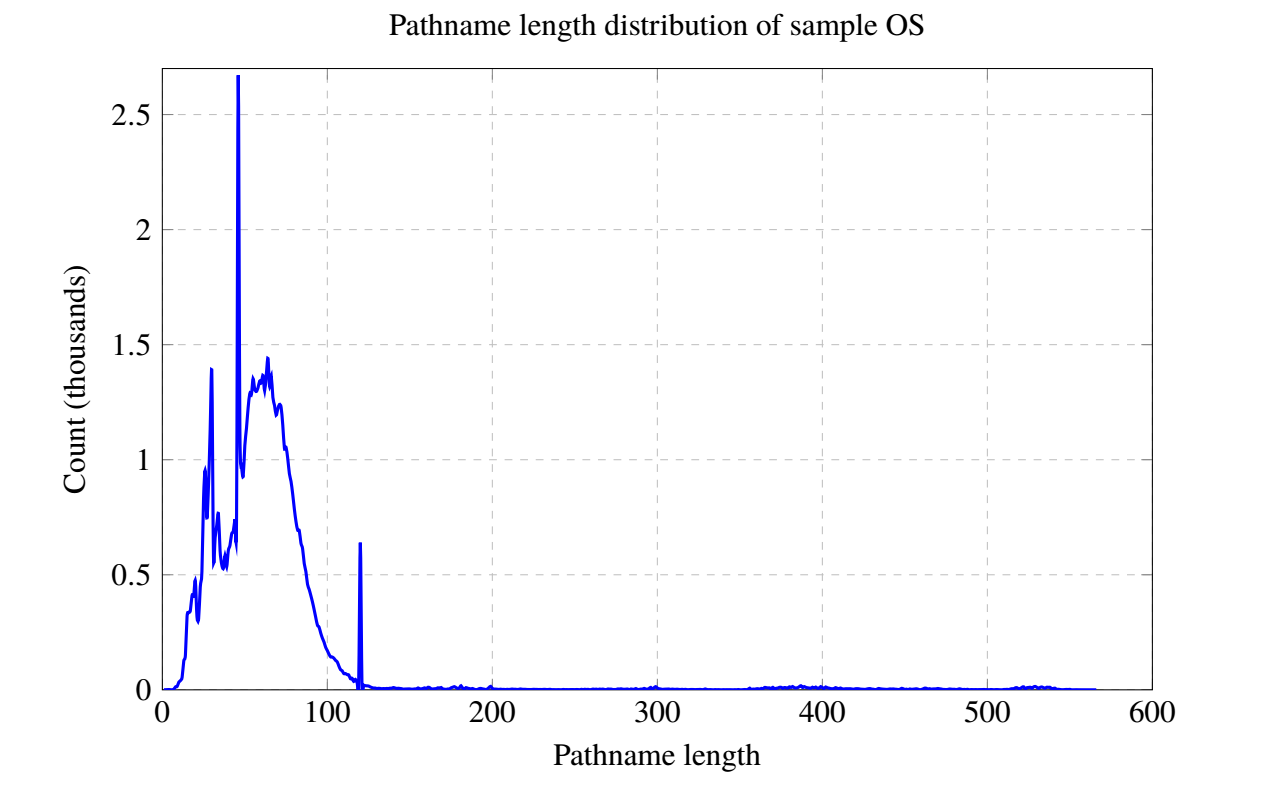
\includegraphics[scale=0.45]{images/graph1.png}
%	\caption{Pathname length count}
%	\label{fig:pathname_length}
%\end{figure}
%
%
%\subsection{Full \ac{OS} \ac{SACL} performance overhead}
%
%\par Finally, we wanted to evaluate whether \emph{Ferify} can be used on the whole filesystem of a guest \ac{OS}. To do that we just created a \ac{SACL} that was generated by the aforementioned script when providing as mount-point the root folder of the guest \ac{OS}. Since the vast majority of the files is in the same range of length, we expect significant delays in our script execution.
%



